En cada una de las LANs mencionadas en la sección \ref{sec:introduccion}, utilizamos las herramientas desarrolladas para capturar el tráfico ARP, y posteriormente gráficar y analizar los datos obtenidos. Con la finalidad de reconocer los nodos distinguidos de cada red, realizamos los siguientes tres tipos de gráficos, representando los conceptos definidos en la sección \ref{sec:desarrollo}.

\subsection{Grafos dirigidos}

  Para representar gráficamente el grafo de relación entre los nodos de una muestra (sección \ref{subsec:grafo-relacion-nodos}), graficamos grafos dirigidos donde hay un nodo por cada IP que aparece en alguno de los paquetes capturados.
 
  Una arista entre los nodos A y B significa que se encontro un paquete con \emph{src} A y \emph{dst} B. El peso de cada arista corresponde a la cantidad de paquetes de la forma anterior.
  
  Por ejemplo, en la figura \ref{fig:FedeGrafo-ejemplo}, se observó un paquete con fuente \emph{192.168.1.12} y destino \emph{192.168.1.1}, y un total de 12 paquetes con fuente \emph{192.168.1.1} y destino \emph{192.168.1.5}.
  
  \begin{figure}[H]
  \begin{center}
    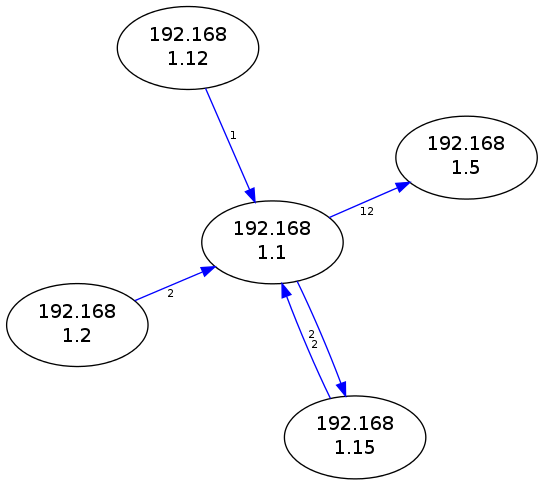
\includegraphics[width=0.3\linewidth]{../imgs/red-hogarena_red.png}
    \caption{Grafo de LAN hogareña}
    \label{fig:FedeGrafo-ejemplo}
  \end{center}
\end{figure}

\subsection{Histogramas}

  En cada red y para cada una de las fuentes ($S_{src}$, $S_{dst}$), realizamos un histograma que muestra la cantidad de apariciones de un determinado IP en la fuente. Se muestra un ejemplo en la figura \ref{fig:histograma-entrepiso-dc-s-src-ejemplo}.
  
  \begin{figure}[H]
  \begin{center}
    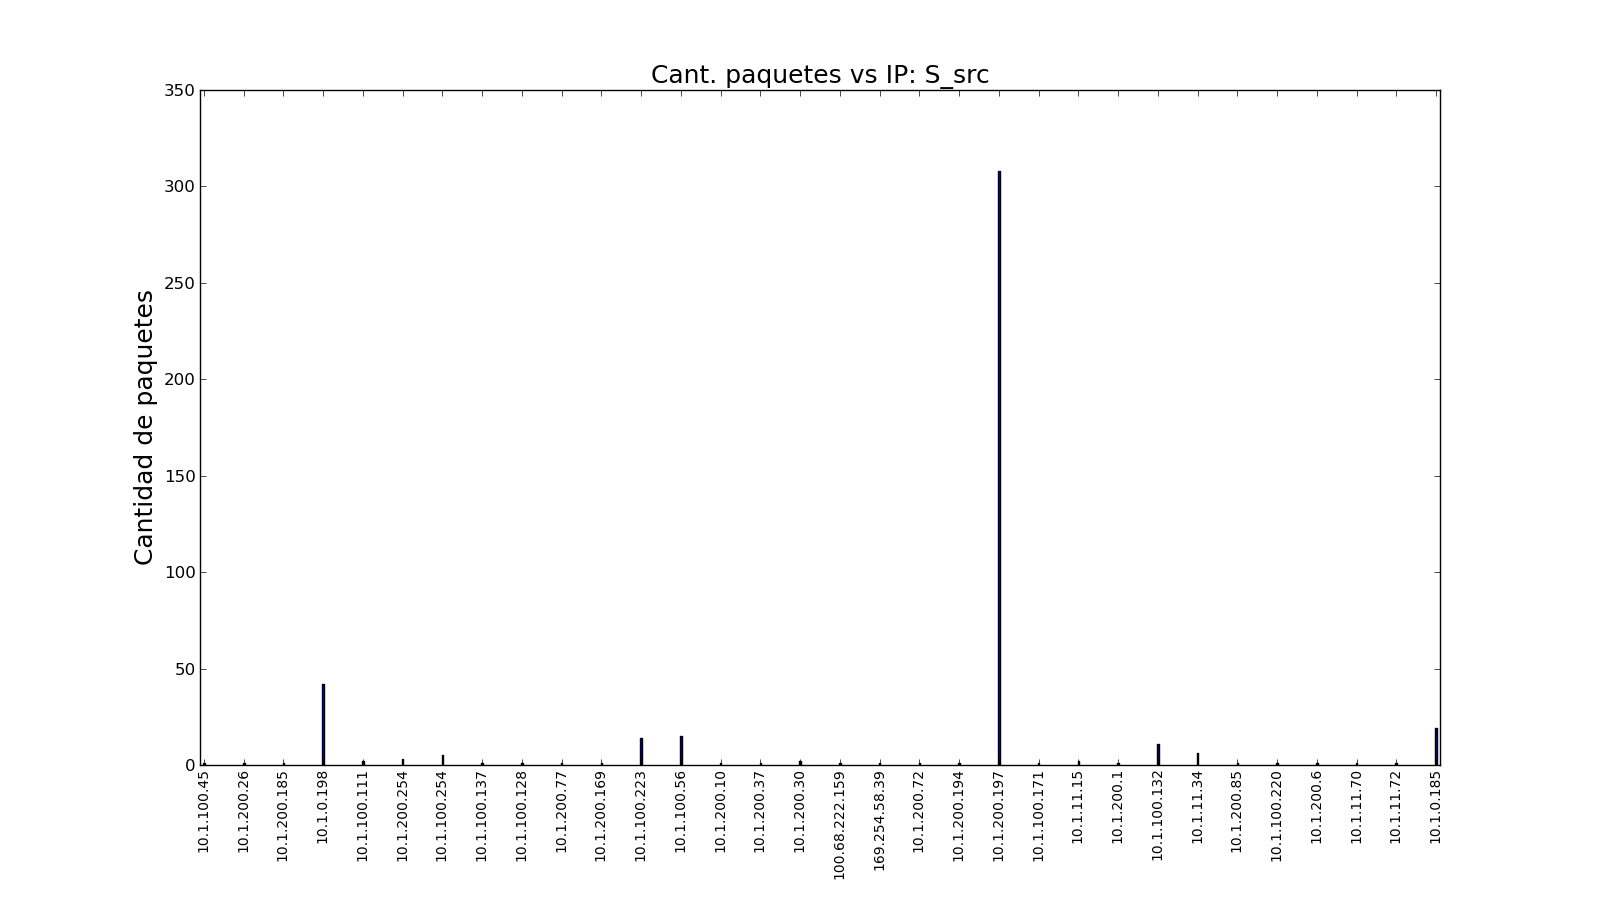
\includegraphics[width=0.8\linewidth]{../imgs/red-entrepiso-dc_S_src_hist.png}
    \caption{Histograma de la serie de paquetes s\_src de la red \emph{Entrepiso-DC}.}
    \label{fig:histograma-entrepiso-dc-s-src-ejemplo}
  \end{center}
  \end{figure}
  
\subsection{Gráficos de información}

  En cada red y para cada una de las fuentes ($S_{src}$, $S_{dst}$), realizamos un gráfico donde se muestra la información de la aparición de un determinado IP en la fuente. Además, graficamos una recta (en rojo) mostrando el valor de la entropía de la fuente, para comparar fácilmente la información de cada IP con la entropía de la fuente. Se muestra un ejemplo en la figura \ref{fig:informacion-entrepiso-dc-s-src-ejemplo}.
  
  \begin{figure}[H]  
  \begin{center}
    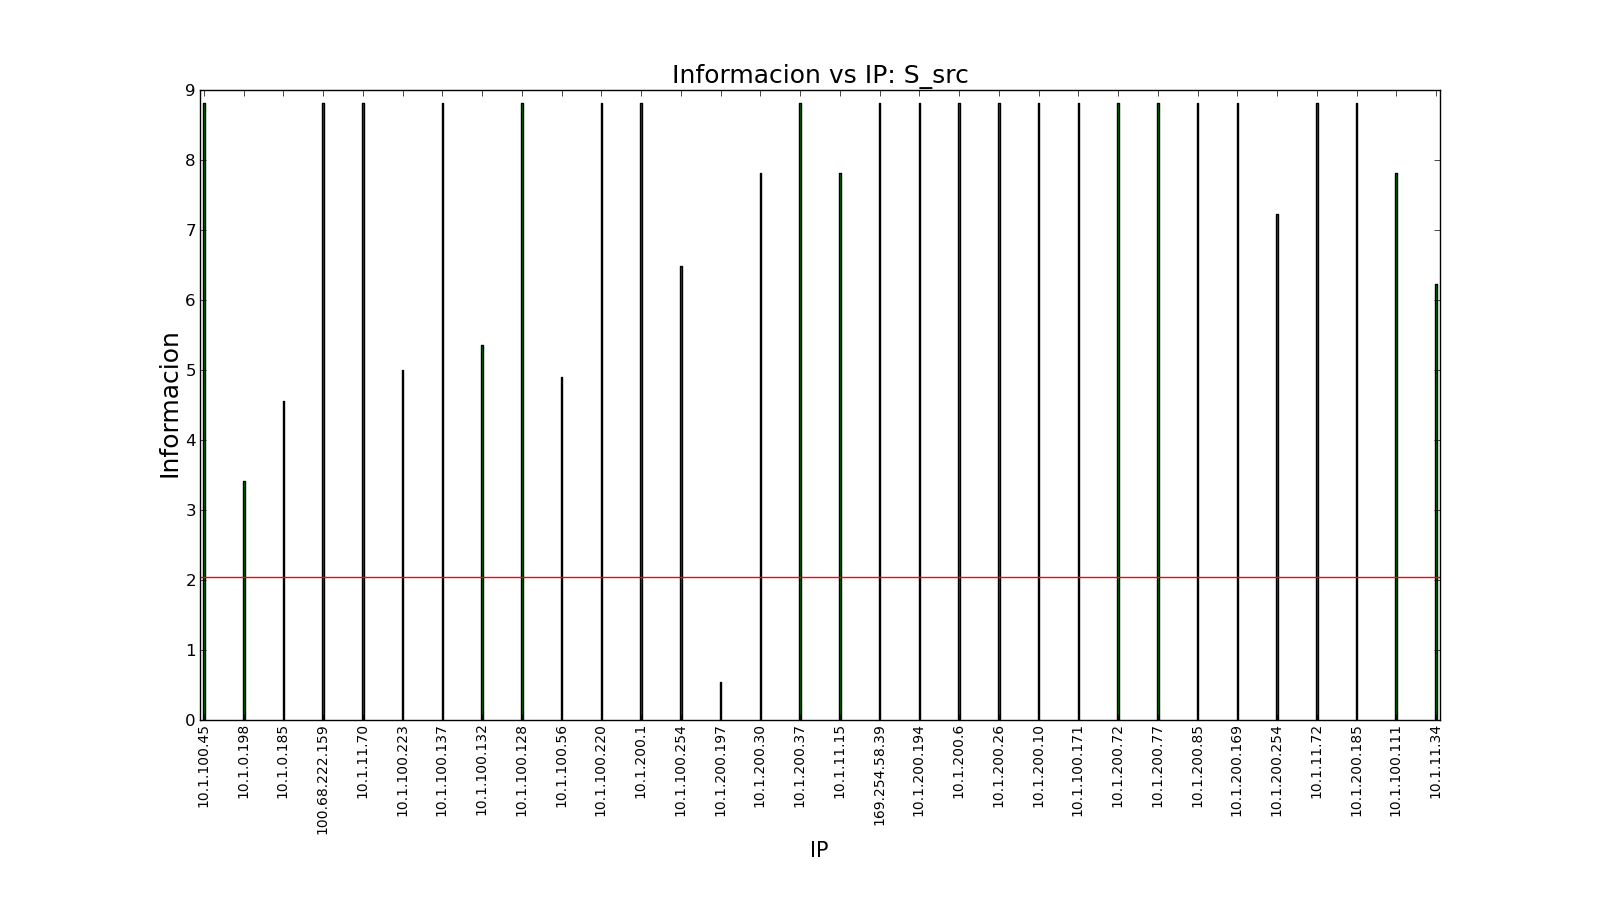
\includegraphics[width=0.8\linewidth]{../imgs/red-entrepiso-dc_S_src_info.png}
    \caption{Gráfico de cantidad de información para cada IP s\_src de la red \emph{Entrepiso-DC}.}
    \label{fig:informacion-entrepiso-dc-s-src-ejemplo}
  \end{center}
\end{figure}